\documentclass[twocolumn]{article}
\usepackage[a4paper, top=2cm, bottom=2cm, left=2cm, right=2cm]{geometry}
\usepackage[onehalfspacing]{setspace}
\usepackage{amsmath}
\usepackage{amssymb}
\usepackage{graphicx}
\usepackage{kotex}
\usepackage{hyperref}
\title{물에 잠긴 연필이 그리는 별 모양의 곡선:\\ 일상 속에 숨어 있는 빛의 기하학}
\author{M. Ryu \\ {\href{mailto:mingshey@hafs.hs.kr}{mingshey@hafs.hs.kr}}}
\begin{document}
\maketitle
\newcommand{\romana}{{a}}
\newcommand{\romanb}{{b}}
\newcommand{\romanA}{{A}}
\newcommand{\romanB}{{B}}
\newcommand{\greeka}{{\alpha}}
\newcommand{\greekb}{{\beta}}
\newcommand{\Aprime}{{A^{\prime}}}
\newcommand{\Bprime}{{B^{\prime}}}
\renewcommand{\figurename}{그림}
\section{서론}

물에 부분적으로 잠긴 연필이 꺾여 보이는 현상은 빛의 굴절을 학습하는 초기 단계에서 흔히 접하는 현상이다(\figurename\ \ref{fig:pencil}). 그러나 연필 끝의 겉보기 위치가 관측 각도에 따라 변화하는 현상은 좀 더 심층적인 분석이 필요하다. 

\begin{figure}[ht]
	\centering
	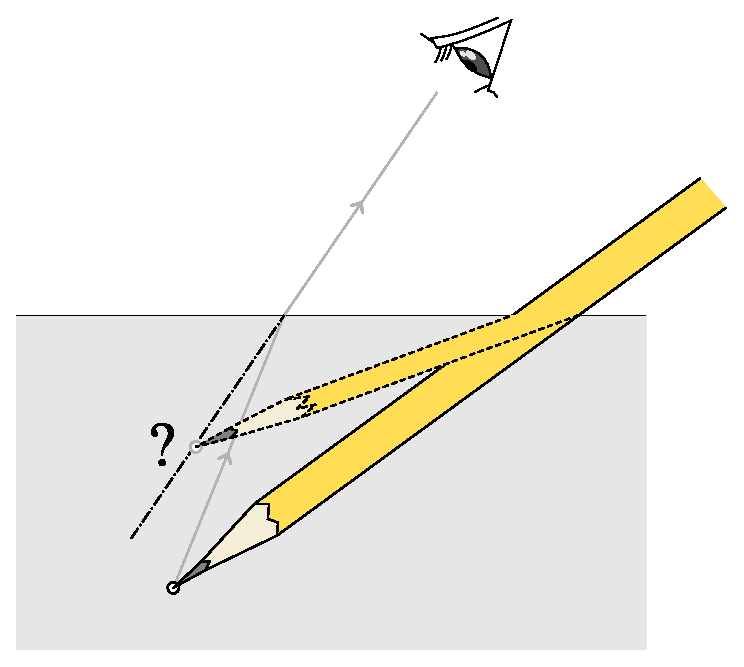
\includegraphics[width=2in]{figs/g164.eps}
	\caption{물 속에서 꺾여 보이는 연필}
	\label{fig:pencil}
\end{figure}

일반적으로 물리학 입문 과정에서는 수직 방향에서 관찰한 겉보기 깊이에 대해 다루지만, 사선 방향에서 관찰했을 때의 겉보기 위치 변화에 대한 상세한 논의는 생략되는 경우가 많다. 고급 광학 교재에서도 이러한 현상은 간략하게 언급되거나 생략되는 경우가 많다. 

이는 이 현상이 수학적인 어려움으로 인해 입문 과정에서 다루기에도 적절하지 않고, 렌즈나 거울과 같은 광학 기기의 작동 원리에 비해 상대적으로 중요성이 낮게 평가되기 때문에 고급 과정에도 어울리지 않기 때문일 것이다. 

하지만 이처럼 단순해 보이면서도 흥미로운 현상이 가끔은 호기심을 자극한다. 필자 외에도 많은 사람이 이 현상을 궁금하게 생각했을 것이다. 본 글에서는 이러한 궁금증에 대한 해답을 제시하고자 한다.


\section{간단한 해답}

호기심은 있지만 시간을 많이 할애하기 어려운 독자를 위해 결론부터 말하자면 이렇다:  
평평한 수면 아래의 점 물체를 수면 위에서 바라볼 때, 상의 위치는 시점(POV)에 따라 달라진다. 
시점이 움직임에 따라 법평면 내에서 관찰되는 상의 자취는 일종의  코스틱(caustic)\footnote{허상의 
자취이므로 `허코스틱'(\emph{virtual caustic}) 이라고 할 수 있겠다.}인데, 이 경우에 
코스틱은 `찌그러진 아스트로이드'라고 불리는 곡선이다.
	
\begin{figure}
	\centering
	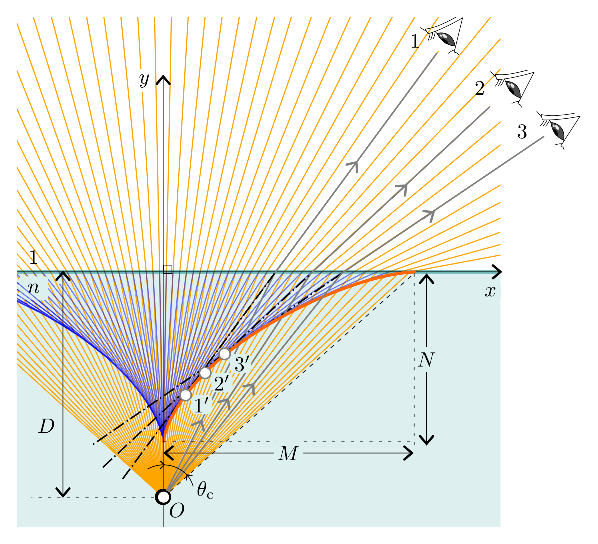
\includegraphics[width=3in]{figs/g409.eps}
	\caption{시점에 따라 위치가 달라지는 상의 자취}
	\label{fig:caustic}
\end{figure}

물체와 시점을 포함하는 법평면에서, \figurename\ \ref{fig:caustic}\과 같이 법평면과 수면의 교선을 $x$-축으로, 
물체를 통과하는 법선을 $y$-축으로 하자. 그러면 상의 자취는 다음 곡선의 일부이다.
	$$ \left| \dfrac{x}{M} \right| ^ {2/3} 
	+ \left| \dfrac{y}{N} \right| ^ {2/3} = 1,$$
여기서 $M = D/\sqrt{n^2 - 1}$은 전반사의 임계각($\theta_{\mathrm{c}}$)에 의해 결정되는 입사 거리의 최댓값이고, 
$N = D/n$은 바로 위에서 관찰할 때 물체의 겉보기 깊이이며, 
$D$는 물체의 실제 깊이이고, $n$은 공기에 대한 물의 굴절률이다.
	
\section{공식의 유도}
	
공기와 물의 굴절률을 각각 $n_1$ 및 $n_2$라고 하자. 공기와 물의 경계면 아래 깊이 $D$인 곳에 점 물체 $O$가 있다. 
물체에서 출발한 광선이 $y$-축으로부터 $\romana$만큼 떨어진 경계면 위의 점 A에 
법선으로부터 $\theta_2$의 각도로 입사한 후, 동일한 법선으로부터 $\theta_1$의 각도로 공기 중으로 굴절된다.

입사각 $\theta_2$가 변할 때 굴절광선 ${\mathrm{AB}}$들이 중첩하여 포락선을 형성하는데, 이렇게 광선들이 모여 만드는 포락선을 코스틱이라고 한다.\footnote{이 경우에는 실제 광선들이 아닌 광선들의 연장선이 만드는 가상의 코스틱, 즉 허코스틱이다.} 상은 선분 ${\mathrm{AB}}$와 코스틱의 접점 $\mathrm{C}$에 위치한다. 
이는 이 점 근처의 광선 다발이 국지적으로 발산하는 점이기 때문이다. 

\begin{figure}
	\centering
	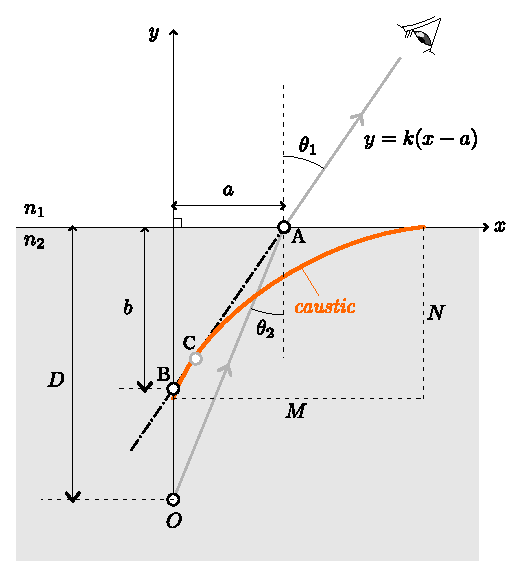
\includegraphics[width=3in]{figs/g237.eps}
	\caption{물-공기 경계면에서 굴절하는 광선 및 그 연장선과 코스틱의 기하학적 관계}
	\label{fig:geometry}
\end{figure}

스넬의 법칙에 의해 다음의 관계식을 얻을 수 있다.
$$ \sin\theta_1 = \frac{n_2}{n_1} \sin\theta_2 = n\sin\theta_2.$$
굴절된 광선의 연장선은 다음 방정식으로 표현된다.
$$y=k(x-\romana).$$

여기서 스넬의 법칙을 고려하면,
$$k=\dfrac{1}{\tan\theta_1}=\dfrac{\cos\theta_1}{\sin\theta_1}
	=\dfrac{\sqrt{1-n^2\sin^2\theta_2}}{n\sin\theta_2}.$$
기하학적으로 다음 관계가 성립한다:
$$\romana = D\tan\theta_2 = \dfrac{D\sin\theta_2}{\cos\theta_2}.$$
직선이 $y$-축과 만나는 점을 B($y=\romanb$)라 하면,
$$\begin{aligned}
	\romanb &= -k\romana \\
	&= -\dfrac{D\sin\theta_2}{\cos\theta_2}
	\dfrac{\sqrt{1-n^2\sin^2\theta_2}}{n\sin\theta_2}\\
	&=-\dfrac{D\sqrt{1-n^2\sin^2\theta_2}}{n\cos\theta_2}.
\end{aligned}$$

이제, 무차원 파라미터 $\greeka=\romana/M$ 및 $\greekb=\romanb/N$를 도입하면,

$$ \begin{aligned}
	\greeka^2 + \greekb^2 &= \dfrac{\romana^2}{M^2}+\dfrac{\romanb^2}{N^2}\\
	&=\dfrac{n^2-1}{D^2}\dfrac{D^2\sin^2\theta_2}{\cos^2\theta_2}%
	+\dfrac{n^2}{D^2}\dfrac{D^2(1-n^2\sin^2\theta_2)}{n^2\cos^2\theta_2}\\
	&=\dfrac{\left(n^2-1\right)\sin^2\theta_2 + 1-n^2\sin^2\theta_2}
	{\cos^2\theta_2}\\
	&=\dfrac{1-\sin^2\theta_2}{\cos^2\theta_2}\\
	&= 1
\end{aligned}$$
%
이고, 역시 무차원 좌표 $\xi=x/M$ 및 $\eta=y/N$를 도입하면, 시점이 $xy$-평면에서 움직임에 따라 점 $\mathrm{\romanA}(\romana, 0)$와 $\mathrm{\romanB}(0, \romanb)$도 움직이는데, 점 $\mathrm{\romanA}$, $\mathrm{\romanB}$ 각각에 대응되는  $\xi\eta$-평면의 점 $\mathrm{\Aprime}(\greeka, 0)$
와 $\mathrm{\Bprime}(0, \greekb)$는 거리를 $1$로 일정하게 유지하며 움직인다.

매개변수를 $\alpha$로 하는 선분 ${\mathrm{\Aprime\Bprime}}$들을 중첩시켰을 때 형성되는 포락선은 `아스트로이드'(%
\href{https://en.wikipedia.org/wiki/Astroid}{\emph{astroid}}\footnote{
소행성을 뜻하는 \emph{asteroid}와 혼동하지 말 것.})라 불리는 잘 알려진 곡선인데, 아스트로이드는 다음 방정식으로 표현된다.
$$ \left| \xi \right|^{2/3} + \left| \eta \right|^{2/3} = 1. $$

\begin{figure}
	\centering
	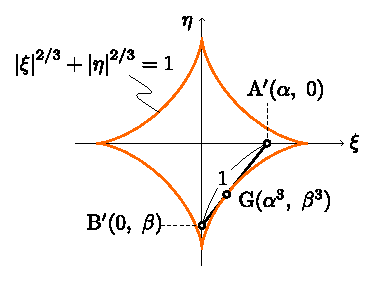
\includegraphics{figs/g107.eps}	
	\caption{코스틱을 $\xi\eta$ 평면에 투영한 모습은 아스트로이드이다.}
	\label{fig:astroid}
\end{figure}

선분 ${\mathrm{\Aprime\Bprime}}$과
아스트로이드의 접점은 $\mathrm{G}(\greeka^3, \greekb^3)$인데, 이 점이 상의 위치 $\mathrm{C}$에 대응되는 점이다.
	
따라서 다음 관계식으로부터 상의 좌표 $(x_{\mathrm{C}}^{}, y_{\mathrm{C}}^{})$를 얻을 수 있다.
$$ \left\{ 
\begin{aligned}
	\xi_{\mathrm{G}}^{} &= \dfrac{x_{\mathrm{C}}^{}}{M} = \greeka^3 = \dfrac{\romana^3}{M^3},\\
	\eta_{\mathrm{G}}^{} &= \dfrac{y_{\mathrm{C}}^{}}{N} = \greekb^3 = \dfrac{\romanb^3}{N^3}.
\end{aligned}
\right.$$
즉,
$$ \left\{ 
\begin{aligned}
	x_{\mathrm{C}}^{} &= \dfrac{\romana^3}{M^2},\\
	y_{\mathrm{C}}^{} &= \dfrac{\romanb^3}{N^2}=-\dfrac{k^3\romana^3}{N^2}.
\end{aligned}
\right.$$

여기서
	$$\sin\theta_2 = \dfrac{\romana}{\sqrt{D^2+\romana^2}}$$
를 이용하여
$$k = \dfrac{\sqrt{D^2-(n^2-1)\romana^2}}{n\romana},$$
를 얻을 수 있으며, 
상의 위치를 $\romana$에 대한 매개변수 함수로 유도할 수 있다.
$$ \left\{ 
\begin{aligned}
	x_{\mathrm{C}}^{} &= (n^2-1)\dfrac{\romana^3}{D^2},\\
	y_{\mathrm{C}}^{} &= -\dfrac{n^2}{D^2}\dfrac{\romana^3}
	{n^3\romana^3}\left\{ D^2-(n^2-1)\romana^2 \right\}^{3/2}\\
	&= -\dfrac{D}{n}\left\{ 1-(n^2-1)\dfrac{\romana^2}{D^2} \right\}^{3/2}.
\end{aligned}
\right.$$
	
\section{시점이 물 속에 있는 경우}

물체가 경계면 위 높이 D인 공기 중에 있고, 
시점이 물 속에 있는 경우, 상대적인 굴절률은 $1/n < 1$이고, 
유사한 추론에 의해 코스틱에 대한 다음 방정식을 얻는다.
$$ \left| \xi \right|^{2/3} - \left| \eta \right|^{2/3} = -1, $$
여기서 $\xi = \dfrac{x}{W} $ 및 $\eta = \dfrac{y}{Z}$이고, 
$W = \dfrac{nD}{\sqrt{n^2-1}}$ 및 $Z = nD$인데,  이 곡선은 점근선을 가지지는 않지만 $x\rightarrow\pm\infty$일 때 기울기가 $\pm Z/W = \pm \sqrt{n^2-1}$에 수렴한다.

따라서 물 속에서 본 물 위 하늘의 풍경은
연직선으로부터 전반사의 임계각 안쪽 원(또는 원뿔) 안에 압축되어 보인다. 이것은 
`스넬의 창'(Snell's window)이라고 하는 잘 알려진 현상이며 전천 사진과 같은 초광각 
사진에 사용되는 어안렌즈(fisheye lens)의 시야와도 닮았다.

이 곡선의 좀 더 일반적인 형태는 
$$ \left| \xi \right|^{r} - \left| \eta \right|^{r} = \pm1 $$
인 곡선들의 계열인데, \href{http://dynamicmathematicslearning.com/super-ellipse.html}%
{DML}\footnote{\ttfamily{dynamicmathematicslearning.com/super-ellipse.html}}에서는 \emph{Super Hyperbola}라는 이름으로 부르고 있고 
\href{https://old.nationalcurvebank.org/superconicncb/superconicncb.htm}{`National Curve Bank'}\footnote{\ttfamily{old.nationalcurvebank.org/superconicncb/\\superconicncb.htm}}에서는
아스트로이드가 속한 
$$ \left| \xi \right|^{r} + \left| \eta \right|^{r} = 1. $$
와 같이 정의되는 `초타원'(\href{https://mathworld.wolfram.com/Astroid.html}%
{\emph{superellipse}})이라는 곡선 계열과 함께 묶어
`초원뿔곡선'(\emph{superconics}) 이라는 집합적인 명칭으로 부르고 있는, 광범위한 곡선 계열의 일부이다.

특히
$$ \left| \xi \right|^{2/3} - \left| \eta \right|^{2/3} = \pm1 $$
인 특수한 경우는 물 위의 점광원에서 나와 물 속으로 들어가며 굴절된 광선들의 코스틱 곡선으로서 
물리학적으로도 의미가 있고, 아스트로이드에 대한 이 곡선의 관계가 타원에 대한 쌍곡선의 관계와 
비슷하므로, 여기에 `쌍곡-아스트로이드'(\emph{hyperastroid})라고 이름을 붙여보는 것도 좋을 듯하다. 

\begin{figure}
	\centering
	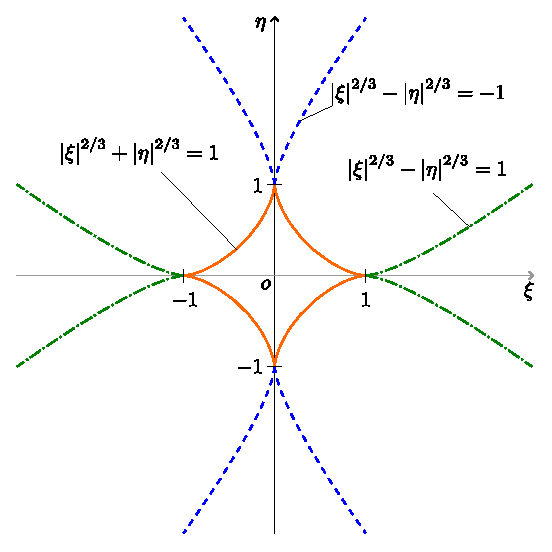
\includegraphics[width=3in]{figs/g254.eps}
	\caption{아스트로이드 및 `쌍곡-아스트로이드'}
	\label{fig:hyperastroid}
\end{figure}

\section{상의 위치 찾기}
물체의 위치와 시점이 주어졌을 때 코스틱을 이용하여 상의 위치를 다음과 같이 찾을 수 있다.

\begin{figure}[ht]
	\centering
	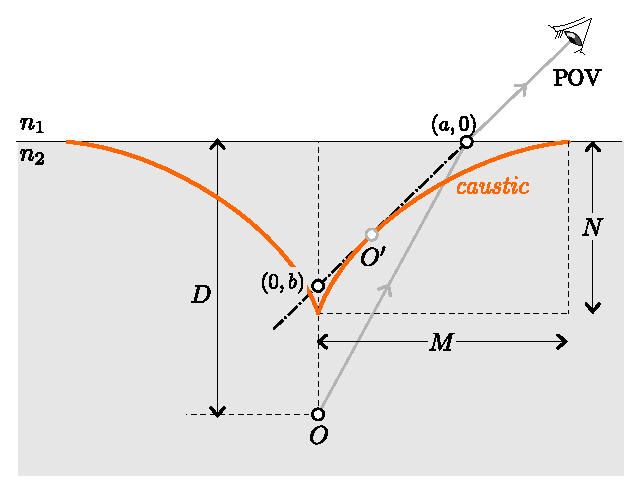
\includegraphics[width=3in]{figs/g394.eps}
	\caption{코스틱을 이용한 상의 위치 결정}
	\label{fig:image_caustic}
\end{figure}

시점에서 코스틱에 접선을 그린다. 접선과 코스틱의 접점이 상의 위치이고, 접선이 수면과 
교차하는 점은 물체에서 나온 광선이 수면에 입사하는 점이다. 
예를 들어 물속에 반쯤 잠긴 연필의 상은 시점에 따라 그림 \ref{fig:pencil_view}\과 같이 달라진다.
\begin{figure}[ht]
	\centering
	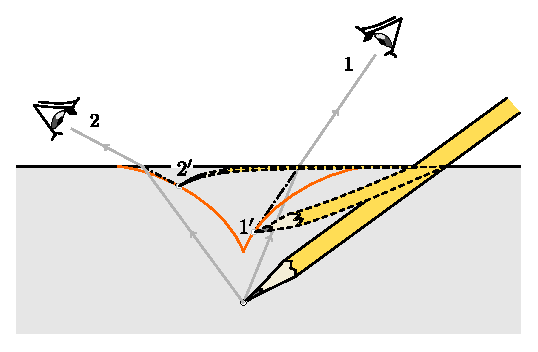
\includegraphics[width=3in]{figs/g43.eps}
	\caption{물에 잠긴 연필의 상은 시점 $1$, $2$에 따라 각각 $1'$, $2'$로 위치와 모양이 달라 보인다.}
	\label{fig:pencil_view}
\end{figure}

물 속에 연속된 물체가 있다면 물체의 표면을 따라 놓인 점 $1, 2, 3, \dots$ 에 대해 
각각 이와 같은 방법으로 상 $1', 2', 3', \dots$을 찾을 수 있다. 점이 연속으로 움직일 때 이에 따라 움직이는 상의 자취가 
물체의 상이 될 것이다.

단, 코스틱에 대한 접선은 해석적으로 찾기 어렵고 실제로는 수치적인 방법을 이용하여 
근삿값을 찾는 것으로 만족해야 할 것이다.

또다른 방법은 물체와 시점을 잇는 광선의 경로를 페르마의 원리를 이용하여 수치적으로 
구한 다음, 광선이 수면과 교차하는 점의 좌표를 바탕으로 아스트로이드의 접점 공식을 이용하여
상의 위치를 구하는 방법이다. 이에 대한 파이썬 예제는  
\href{https://github.com/mingshey/python_projects/blob/main/Refraction_Image.ipynb}%
{\sffamily{github}}\footnote{\ttfamily{https://github.com/mingshey/python\_projects/blob/main/\\Refraction\_Image\_en.ipynb}} 에 공개되어 있다.

\begin{figure}[ht]
	\centering
	\includegraphics*[width=3in]{figs/g240.eps}
	\caption{연속적인 물체의 상}
	\label{fig:extended_image}
\end{figure}

\appendix
\newcommand{\pd}[2]{{\frac{\partial #1}{\partial #2}}}
\newcommand{\ilpd}[2]{{{\partial #1}/{\partial #2}}}
\section*{부록: 포락선으로 정의한 아스트로이드}
평면 상의 직교 좌표에서 $x$ 축 위의 점  $(a, 0)$과 $y$ 축 위의 점 $(0, b)$가 일정한 거리 $c$를 유지하며 움직인다고 하자. 그러면 $a^2+b^2=c^2$이고, 어느 순간 선분을 포함하는 직선의 방정식을 
$$y=-\dfrac{b}{a}(x-a)$$
라 쓸 수 있다. 여기에 
$b=\pm \sqrt{c^2-a^2}$를 대입하면 
$$y(x, a) = \mp \dfrac{\sqrt{c^2-a^2}}{a}(x-a)$$
라 할 수 있다. 
$a$ 값이 변하면 두 점을 잇는 선분도 변한다. 이러한 선분들의 계열이 이루는 포락선은 $a$가 극소량 변할 때 변하지 않는 정류점, 즉
$\ilpd{y}{a} = 0$인 점들의 자취로 정의할 수 있다. 이 조건을 만족하는 $(x, y)$들을 구하기 위해 $y$를 $a$로 미분하면,

$$ \begin{aligned}
\pd{y}{a} &= \pm\left[\left( \dfrac{1}{\sqrt{c^2-a^2}}+\dfrac{\sqrt{c^2-a^2}}{a^2}\right) (x-a) + \dfrac{\sqrt{c^2-a^2}}{a} \right]\\
	&= \pm \dfrac{(a^2+c^2-a^2)(x-a)+a(c^2-a^2)}{a^2\sqrt{c^2-a^2}}\\
	&= \pm \dfrac{c^2 x - a^3}{a^2 \sqrt{c^2 - a^2}}\\
	&= 0.
\end{aligned}
$$
따라서 정류점의 $x$좌표는 $x = a^3/c^2$ 이고, 이를 다시 $y(x, a)$에 대입하면 $y$좌표의 값은

$$ \begin{aligned}
y(x, a) &= \mp \dfrac{\sqrt{c^2-a^2}}{a}\left(\dfrac{a^3}{c^2}-a\right)\\
	& = \pm \dfrac{\left( c^2- a^2 \right)^{3/2}}{c^2}\\
	& = \dfrac{b^3}{c^2}
\end{aligned}
$$
이다. 따라서 정류점의 좌표 $(x, y)$는 다음 방정식을 만족한다:
$$ \left|\dfrac{x}{c}\right|^{2/3} + \left|\dfrac{y}{c}\right|^{2/3} = 1. $$
$\blacksquare$

%\section*{감사의 글}
%딸들의 세심한 조언 덕분에 이 글을 완성할 수 있었습니다. 감사합니다.

\end{document}